%%%%%%%%%%%%%%%%%%%%%%%%%%%%%%%%%%%%%%%%%%%%%%%%%%%%%%%%%%%%%%%%%%%%%%%%%%%
% Chapter 1: Descriptive statistics
%%%%%%%%%%%%%%%%%%%%%%%%%%%%%%%%%%%%%%%%%%%%%%%%%%%%%%%%%%%%%%%%%%%%%%%%%%%

\Chapter{Chapter 1}{Descriptive statistics}{Chapter 1: Descriptive statistics}{
Please read Chapter 1 (excl. section 1.3), Chapter 2, and Section 5.1-5.6 from \textit{\href{https://learningstatisticswithr.com/}{{\color{black}Learning Statistics with R}}} before starting these assignments.
}
\fancyhead[R]{\fontsize{12}{14}\selectfont\textit{Chapter 1: Descriptive statistics}}

\chaptertitle{Chapter 1: Descriptive statistics}

\learningobjectives{
    \item Calculating the mean, mode, median, quartiles and range by hand 
    \item Get started with \texttt{R}: set the working directory, inspect and load data
    \item Calculating the mean, mode, median and range in R
    \item Demonstrating the Central Limit Theorem in R
}

% To add an assignment to the chapter, create a file in the folder "Assignments" and insert the link below

%%%%%%%%%%%%%%%%%%%%%%%%%%%%%%%%%%%%%%%%%%%%%%%%%%%%%%%%%%%%%%%%%%%%%%%%%%%
% Assignment 1.1: Descriptive statistics by hand
%%%%%%%%%%%%%%%%%%%%%%%%%%%%%%%%%%%%%%%%%%%%%%%%%%%%%%%%%%%%%%%%%%%%%%%%%%%

\handassignment{Assignment 1.1: Descriptive statistics by hand}


Calculate by hand (or by the use of a pocket calculator) the

\begin{itemize}
    \item \concept{mean} 
    \item \concept{mode}
    \item \concept{median}
    \item \concept{range}
    \item \concept{lower and upper quartiles}
    \item \concept{interquartile range}
\end{itemize}

For the following data sets: \\

\question{
    1.1 a
}{
    2\hspace{.3cm}7\hspace{.3cm}4\hspace{.3cm}5\hspace{.3cm}8\hspace{.3cm}10\hspace{.3cm}10\hspace{.3cm}7\hspace{.3cm}9\hspace{.3cm}2\hspace{.3cm}8\hspace{.3cm}8\hspace{.3cm}9\hspace{.3cm}4\hspace{.3cm}6
}
\vspace*{-.4cm} \\
\question{
    1.1 b
}{
    7\hspace{.3cm}7\hspace{.3cm}6\hspace{.3cm}5\hspace{.3cm}2\hspace{.3cm}1\hspace{.3cm}3\hspace{.3cm}7\hspace{.3cm}5\hspace{.3cm}9\hspace{.3cm}9\hspace{.3cm}10
}

\emptyanswerbox{
1.1a
}{ 
Mean: \quad \shortanswerline \hspace{.5cm} \quad Range: \qquad \qquad \qquad \qquad \shortanswerline
            \answerbreak
            Mode: \quad \shortanswerline \hspace{.4cm} \quad Lower quartile: \qquad \quad \shortanswerline
            \answerbreak
            Median: \shortanswerline \hspace{.4cm} \quad Upper quartile: \qquad \quad \shortanswerline
            \answerbreak
            \hspace*{6.1cm} \quad Interquartile range: \shortanswerline}
            
\emptyanswerbox{
1.1b
}{  Mean: \quad \shortanswerline \hspace{.5cm} \quad Range: \qquad \qquad \qquad \qquad \shortanswerline
            \answerbreak
            Mode: \quad \shortanswerline \hspace{.4cm} \quad Lower quartile: \qquad \quad \shortanswerline
            \answerbreak
            Median: \shortanswerline \hspace{.4cm} \quad Upper quartile: \qquad \quad \shortanswerline
            \answerbreak
            \hspace*{6.1cm} \quad Interquartile range: \shortanswerline}

\clearpage % Page break

\question{
    1.1 c
}{
    Describe which question (1.1a or 1.1b) was more difficult to calculate and why.
}

\fourlineanswerbox{1.1c} 

\question{
    1.1 d
}{
    Are these data sets \concept{positively skewed} or \concept{negatively skewed}? Circle the correct answer and explain why you chose this answer using the relation between the \concept{mean}, the \concept{median}, and the \concept{mode}.
}

\emptyanswerbox{
1.1d
}{
These data sets are \textbf{positively} / \textbf{negatively} skewed.
\answerskip
Explanation:
\answerskip
\rule{\textwidth}{0.4pt}
\answerbreak
\rule{\textwidth}{0.4pt}
\answerbreak
\rule{\textwidth}{0.4pt}
}

\clearpage % Page break 
%%%%%%%%%%%%%%%%%%%%%%%%%%%%%%%%%%%%%%%%%%%%%%%%%%%%%%%%%%%%%%%%%%%%%%%%%%%
% Assignment 1.2: Descriptive statistics of small data sets in R
%%%%%%%%%%%%%%%%%%%%%%%%%%%%%%%%%%%%%%%%%%%%%%%%%%%%%%%%%%%%%%%%%%%%%%%%%%%

\rassignment{Assignment 1.2: Descriptive statistics of small data sets in R}

This assignment assumes you opened a new script in the code editor in
\texttt{RStudio}. Write and run your own code to answer the following questions. \\

In R, a one-dimensional row of numbers is represented by a \rcode{vector}. \\

\question{
    1.2 a
}{
    Use the \rcode{c()} function to enter the numbers from assignment 1.1a in a new vector called \rcode{dataset1}. Next, run the following code in \texttt{R} and explain what you see.
}

\codeblock{View(dataset1)}

\hint{Hint 1.1: Check Part I of the R help for more information on how to make a \rcode{vector}.}

\rcodeanswersmall{1.2a}
\twolineanswerbox{1.2a}

\question{
    1.2 b
}{
    Write and run your own code in R to find the \concept{mean}, \concept{mode}, \concept{median}, and \concept{range} for the vector \rcode{dataset1}. Compare your answers with those of assignment 1.1a.
}

\hint{Hint 1.2: Check part IV of the R help on page~\pageref{rhelp} for descriptive statistics functions.}
\hint{Hint 1.3: There is no \concept{mode} function in R, but you can find the mode in a frequency \rcode{table}.}

\rcodeanswersmall{1.2b}

\clearpage % Page break

\emptyanswerbox{
1.2b
}{  Mean: \quad \shortanswerline \hspace{.5cm} \quad Median: \quad \quad \shortanswerline
            \answerskip
            Mode: \quad \shortanswerline \hspace{.5cm} \quad Range: \qquad \quad \shortanswerline}

\question{
    1.2 c
}{
    Run the following code in \texttt{R} and explain what you see.
}

\codeblock{quantile(dataset1, type = 6)}
\twolineanswerbox{1.2c}

\question{
1.2 d
}{
Use the \rcode{c()} function to create a vector \rcode{dataset2} with the data from assignment 1.1b and find the \concept{mean}, \concept{mode}, \concept{median}, \concept{range}, and \concept{quartiles} for these data. Compare your answers with those of assignment 1.1b.
}

\rcodeanswersmall{1.2d}

\emptyanswerbox{
    1.2d
}{  
Mean: \quad \shortanswerline \hspace{.5cm} \quad Range: \qquad \qquad \qquad \qquad \shortanswerline
            \answerbreak
            Mode: \quad \shortanswerline \hspace{.4cm} \quad Lower quartile: \qquad \quad \shortanswerline
            \answerbreak
            Median: \shortanswerline \hspace{.4cm} \quad Upper quartile: \qquad \quad \shortanswerline
}
            
\clearpage % Page break
%%%%%%%%%%%%%%%%%%%%%%%%%%%%%%%%%%%%%%%%%%%%%%%%%%%%%%%%%%%%%%%%%%%%%%%%%%%
% Assignment 1.2: Descriptive statistics of larger data sets in R
%%%%%%%%%%%%%%%%%%%%%%%%%%%%%%%%%%%%%%%%%%%%%%%%%%%%%%%%%%%%%%%%%%%%%%%%%%%

\rassignment{Assignment 1.3: Descriptive statistics of larger data sets in R}

For this assignment, you need the \dataset{bloodPressure.csv} data set that you can download from the online resources. This data set contains measurements of the age, blood pressure, cholesterol level, gender, and description of a random selection of people. It is normally used to look for relationships between these variables. Note that this is fake data and does not contain actual measurements. \\

Let’s start with importing the data set (which is available in the online resources) into \texttt{R}. \\

\question{
    1.3 a
}{
    Inspect and run the following code in \texttt{R} to import the blood pressure data and store it in the object \rcode{dataset3}. Explain how the code works and describe what the \dataset{bloodPressure.csv} file contains.
}

\codeblock{dataset3 <- read.csv(file.choose())}
\twolineanswerbox{1.3a}

This method of importing data can be a lot of work if there are many files or if the script will be run many times. Faster methods exist though, for example by providing the full file path. \\

\question{
    1.3 b
}{
    Describe and test ways this code can be improved to make importing a file easier.
}

\hint{Hint 1.4: Look at Part I of the R help to find out more functions for importing data.}

\twolineanswerbox{1.3b} \\
\rcodeanswersmall{1.3b}

\clearpage % Page break

The functions you used for descriptive statistics on the small data sets in assignment 1.1 can also be applied to the data set that is currently stored in \rcode{dataset3}. \\

\question{
    1.3 c
}{
    Find the \concept{mean}, \concept{mode}, \concept{median}, \concept{range}, and \concept{quartiles} for the column \rcode{Age} in \rcode{dataset3}. Describe this variable in running text using these statistics.
}

\hint{Hint 1.5: First find out how to extract (index) a specific column in a data frame using the \rcode{\$} sign.}

\rcodeanswermedium{1.3c}
\fourlineanswerbox{1.3c}

For large data sets, it becomes a lot of work finding the \concept{mode} in a frequency table each time. It is possible to import a package into the \texttt{R} session that contains a function for calculating the \concept{mode} automatically. However, it is also possible to create a function that calculates the \concept{mode} ourselves. \\

Run the following lines of \texttt{R} code together: \\

\codeblock{getMode <- function(x)\{ \\
  \hspace*{10pt} uniqx <- unique(x) \\
  \hspace*{10pt} uniqx[which.max(tabulate(match(x, uniqx)))] \\
\}
}

You have now created your first \texttt{R} function and you will see it displayed separately in the \texttt{R} environment. This function will give you the \concept{mode} for any \textbf{numeric} vector or column. It works by first extracting all unique values, counting their frequency, and then selecting the value with the highest frequency. Note that you can use this function, but will not be required to understand or make functions like this. However, for the interested reader, part III of the R help contains more information on how to create your own functions. \\

\clearpage % Page break

\question{
    1.3 d
}{
    Use the new \rcode{getMode()} function to determine the \concept{mode} for column \rcode{Age} in \rcode{dataset3} and check if it is consistent with your answer for assignment 1.3c.
}

\rcodeanswertiny{1.3d}
\emptyanswerbox{
    1.3d
}{
    Mode: \shortanswerline
}

\question{
    1.3 e
}{
    Find the \concept{mean}, \concept{mode}, \concept{median}, \concept{range}, and \concept{quartiles} for the column \rcode{BloodPressure} in \rcode{dataset3}. Also use the new \rcode{getMode()} function.
}

\rcodeanswermedium{1.3e}
\emptyanswerbox{
    1.3e
}{
    Mean: \quad \shortanswerline \hspace{.5cm} \quad Range: \qquad \qquad \qquad \qquad \shortanswerline
            \answerbreak
            Mode: \quad \shortanswerline \hspace{.4cm} \quad Lower quartile: \qquad \quad \shortanswerline
            \answerbreak
            Median: \shortanswerline \hspace{.4cm} \quad Upper quartile: \qquad \quad \shortanswerline
}

\question{
    1.3 f
}{
    Is the distribution of the values in the \rcode{BloodPressure} column \concept{positively skewed} or \concept{negatively skewed}? Explain your answer using the relation between the \concept{mean}, \concept{median}, and \concept{mode}.
}

\emptyanswerbox{
1.1f
}{
These data sets are \textbf{positively} / \textbf{negatively} / \textbf{not} skewed.
\answerskip
Explanation:
\answerskip
\rule{\textwidth}{0.4pt}
\answerbreak
\rule{\textwidth}{0.4pt}
\answerbreak
\rule{\textwidth}{0.4pt}
}

\clearpage

\question{
    1.3 g
}{
    Determine the \concept{variance} and \concept{standard deviation} for the column \rcode{Cholestrol} in \rcode{dataset3}.
}

\rcodeanswersmall{1.3g}
\emptyanswerbox{
    1.3g
}{
    Variance: \qquad \qquad \qquad \shortanswerline
    \answerskip
    Standard deviation: \shortanswerline
}

\question{
    1.3 h
}{
    Validate the relation between the \concept{variance} and the \concept{standard deviation} by performing a calculation in \texttt{R}.
}

\rcodeanswertiny{1.3h}

\clearpage % Page break

\setcounter{chapter}{1}
\setcounter{section}{4}
\setcounter{question}{0}

%%%%%%%%%%%%%%%%%%%%%%%%%%%%%%%%%%%%%%%%%%%%%%%%%%%%%%%%%%%%%%%%%%%%%%%%%%%
% Assignment 1.4: Demonstrating the Central Limit Theorem in R
%%%%%%%%%%%%%%%%%%%%%%%%%%%%%%%%%%%%%%%%%%%%%%%%%%%%%%%%%%%%%%%%%%%%%%%%%%%

\rassignment{Demonstrating the Central Limit Theorem in R}

The \concept{normal distribution} is important in statistics because many natural phenomena are normally distributed. For example; height, weight, and IQ scores are all distributed according to this bell shaped curve. But it is famous for another reason: the distributions of all \concept{sample means} follows a \concept{normal distribution}. This is useful knowledge because it means that the values in the original population can be distributed in any way, and still the \concept{means} of its samples will be normally distributed. This is called the \concept{Central Limit Theorem}.\\

To gain an understanding of how the \concept{Central Limit Theorem} works, suppose that you have a single die. Each time you roll that die, you can expect to see a value between 1 and 6. The \concept{population mean} $\mu$ (i.e., the sum of the values multiplied by the probability of seeing each value) is calculated as:

\begin{equation*}
    \mu = \frac{1}{6} \times 1 + \frac{1}{6} \times 2 + \frac{1}{6} \times 3 + \frac{1}{6} \times 4 + \frac{1}{6} \times 5 + \frac{1}{6} \times 6 = 3.5
\end{equation*}

Run the following code in \texttt{R} to confirm the population mean: \\

\codeblock{meanValue <- sum(1:6 * (1 / 6))\\
print(meanValue)
}

Now let's roll two dice at the same time. If you roll a 3 on the first die and a 1 on the second die, then the \concept{mean} is $\frac{1}{2} \times 1 + \frac{1}{2} \times 3 = 2$. With that knowledge you can create a matrix which will give you the \concept{mean} for any combination of dice rolls (the values in the square brackets, \rcode{[ ]}, refer to the values obtained from each die). This is done for you below, but you can try to figure out how to recreate this matrix for yourself. \\

\codeblock{\#\#      [,1] [,2] [,3] [,4] [,5] [,6] \\
\#\# [1,]  1.0  1.5  2.0  2.5  3.0  3.5 \\
\#\# [2,]  1.5  2.0  2.5  3.0  3.5  4.0 \\
\#\# [3,]  2.0  2.5  3.0  3.5  4.0  4.5 \\ 
\#\# [4,]  2.5  3.0  3.5  4.0  4.5  5.0 \\ 
\#\# [5,]  3.0  3.5  4.0  4.5  5.0  5.5 \\
\#\# [6,]  3.5  4.0  4.5  5.0  5.5  6.0
}

The \concept{sample mean} of the two dice ranges from 1 to 6. Note that you only see the values 1 and 6 once in the matrix. This is because the only way to get an \concept{sample mean} of 1 is to roll a 1 on our first die and then roll a 1 on our second die as well. In a similar manner, getting an \concept{sample mean} of 6 means you have to roll a 6 on both dice. Compare these \concept{sample means} of 1 and 6 with a \concept{sample mean} of 1.5. There are two ways to obtain a \concept{sample mean} of 1.5. You could roll a 1 on your first die and a 2 on our second die, or you could roll a 2 on our first die and a 1 on our second die. So, there are more ways to get a 1.5 than to get a 1. In fact, the probability of getting a certain value tends to get larger as you get closer to 3.5 (which is the true \concept{mean} of the population). Look at the diagonal entries of the matrix: 3.5 appears six times in the matrix. \\

From the above, you know that when you roll a die, the \concept{mean} score over the long run will be 3.5. Even though 3.5 isn't an actual value that appears on the die, over the long run if you take the \concept{mean} of the values from multiple rolls, you'd get very close to 3.5. This is the \concept{Central Limit Theorem} in action. 

\clearpage % Page break

Run the following \texttt{R} code to try this for yourself: \\

\codeblock{rolls <- 1000000 \\
mean(sample(x = 1:6, size = rolls, replace = TRUE))
}

As you can see, the mean of 1000000 rolls is very close to 3.5. However, this trend continues as you add more dice. What's interesting is that the underlying distribution of the rolls is not normal, it is uniform: there's a $\frac{1}{6}$ chance of seeing each face of a particular die. But the \concept{sample means} are normally distributed. Run the following \texttt{R} code to simulate multiple \rcode{rolls} of multiple \rcode{dice}, calculate their \concept{sample means}, and make a figure of their distribution. If you want to fully understand this code, check out the \texttt{R} help on page~\pageref{rhelp}. \\

\codeblock{roll <- function(rolls, dice)\{ \\
\hspace*{10pt} means <- NULL \\
\hspace*{10pt} for(i in 1:rolls)\{ \\
\hspace*{20pt} means <- c(means, mean(x = sample(1:6, size = dice, replace = TRUE))) \\
\hspace*{10pt} \} \\
\hspace*{10pt} return(means) \\
\} \\
\\
rolls <- 10000 {\color{dataset} \# Number of rolls with each die}\\
dice <- 1 \hspace*{22pt} {\color{dataset} \# Number of dice}\\
\\
data <- roll(rolls, dice) \\
barplot(prop.table(table(data)), \\
\hspace*{40pt} ylim = c(0,1), width = 6/length(table(data)), las = 1) \\
lines(density(data)) 
}

Now gradually increase the number of \rcode{dice} and run the code again several times. Watch what happens to the distribution of the \concept{sample means} as it becomes more tight around 3.5. 

\begin{center}
    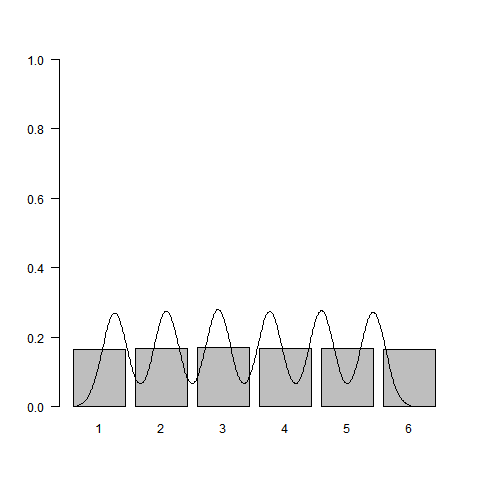
\includegraphics[width=0.3\textwidth]{Files/Images/clm1.png}
    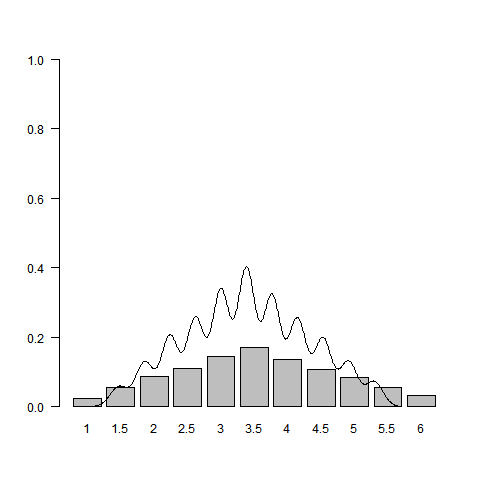
\includegraphics[width=0.3\textwidth]{Files/Images/clm2.png}
    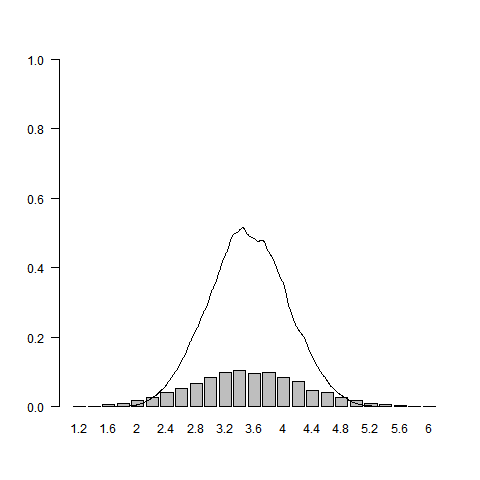
\includegraphics[width=0.3\textwidth]{Files/Images/clm5.png} \\
    \rcode{dice = 1} \hspace{3.3cm} \rcode{dice = 2} \hspace{3.3cm} \rcode{dice = 5}
\end{center}

Saying that the sample distribution becomes more tight around 3.5 as a result of increasing the sample size (the number of \rcode{dice}) can be expressed in a mathematical way:

\begin{equation*}
    \sigma_{\text{sampling distribution}} = \frac{\sigma_{\text{population}}}{\sqrt{n}},
\end{equation*}

where $\sigma$ is the \concept{standard deviation} and $n$ is the size of your sample. So if the sample size is very large, you can expect the \concept{standard deviation} of the \concept{sampling distribution} to be rather small. Important is that the \concept{mean} of the \concept{sampling distribution} is the same as the \concept{population mean}, but the \concept{standard deviation} is not. 

\clearpage % Page break

\vspace*{2cm}
\fancyhf[rh]{}
\begin{center}
    \textit{This page is intentionally left blank}
\end{center}

\clearpage % Page break